%%%%%%%%%%%%%%%%%%%%%%%%%%%%%%%%%%%%%%%%%%%%%%%%%%%%%%%%%%%%%%%%%%%%%%%%%%%%%%%%
%2345678901234567890123456789012345678901234567890123456789012345678901234567890
%        1         2         3         4         5         6         7         8

%\documentclass[journal,transmag]{IEEEtran}% Comment this line out if you need a4paper

\documentclass[10pt, conference]{ieeeconf}      % Use this line for a4 paper

\IEEEoverridecommandlockouts                              % This command is only needed if 
                                                          % you want to use the \thanks command

%\overrideIEEEmargins                                      % Needed to meet printer requirements.

% See the \addtolength command later in the file to balance the column lengths
% on the last page of the document

% The following packages can be found on http:\\www.ctan.org
%\usepackage{graphics} % for pdf, bitmapped graphics files
%\usepackage{epsfig} % for postscript graphics files
%\usepackage{mathptmx} % assumes new font selection scheme installed
%\usepackage{times} % assumes new font selection scheme installed
%\usepackage{amsmath} % assumes amsmath package installed
%\usepackage{amssymb}  % assumes amsmath package installed

\newtheorem{theorem}{Theorem}[section]
\newtheorem{lemma}[theorem]{Lemma}
\newtheorem{proposition}[theorem]{Proposition}
\newtheorem{corollary}[theorem]{Corollary}
\usepackage[ruled,vlined]{algorithm2e}

\newcommand{\qed}{\nobreak \ifvmode \relax \else
      \ifdim\lastskip<1.5em \hskip-\lastskip
      \hskip1.5em plus0em minus0.5em \fi \nobreak
      \vrule height0.75em width0.5em depth0.25em\fi}

\def\lc{\left\lfloor}   
\def\rc{\right\rfloor}

\usepackage{amsmath,amssymb}

\usepackage{tabularx}
\usepackage{tikz,hyperref,graphicx,units}
\usepackage{subfigure}
\usepackage{benktools}

\usepackage{caption}
\usepackage{epstopdf}
\renewcommand{\captionfont}{\footnotesize}
\usepackage{sidecap,wrapfig}
\usepackage[ruled,vlined]{algorithm2e}
\DeclareMathOperator*{\argmin}{arg\,min}
\DeclareMathOperator*{\argmax}{arg\,max}
\newcommand{\abs}[1]{\lvert#1\rvert} 
\newcommand{\norm}[1]{\lVert#1\rVert}
%\newcommand{\suchthat}{\mid}
\newcommand{\suchthat}{\ \big|\ }
\newcommand{\ba}{\mathbf{a}}
\newcommand{\bb}{\mathbf{b}}
\newcommand{\bc}{\mathbf{c}}
\newcommand{\bd}{\mathbf{d}}
\newcommand{\bg}{\mathbf{g}}
\newcommand{\bj}{\mathbf{j}}
\newcommand{\bn}{\mathbf{n}}
\newcommand{\bp}{\mathbf{p}}
\newcommand{\bw}{\mathbf{w}}
\newcommand{\bt}{\mathbf{t}}
\newcommand{\bu}{\mathbf{u}}
\newcommand{\by}{\mathbf{y}}
\newcommand{\bx}{\mathbf{x}}
\newcommand{\bz}{\mathbf{z}}
\newcommand{\bbf}{\mathbf{f}}
\newcommand{\bzero}{\mathbf{0}}
\newcommand{\bG}{\mathbf{G}}
\newcommand{\bA}{\mathbf{A}}
\newcommand{\bW}{\mathbf{W}}
\newcommand{\bX}{\mathbf{X}}
\newcommand{\mX}{\mathcal{X}}
\newcommand{\mD}{\mathcal{D}}
\newcommand{\mG}{\mathcal{G}}
\newcommand{\mN}{\mathcal{N}}
\newcommand{\mW}{\mathcal{W}}
\newcommand{\mF}{\mathcal{F}}
\newcommand{\bZ}{\mathbf{Z}}
\newcommand{\mR}{\mathcal{R}}

\newcommand{\bfc}{W}
\newcommand{\Qinf}{Q_{\infty}}
\newcommand{\st}[1]{_\text{#1}}
\newcommand{\rres}{r\st{res}}
\newcommand{\pos}[1]{(#1)^+}
\newcommand{\depth}{\operatorname{depth}}
\newcommand{\dist}{\operatorname{dist}}
\newcommand{\convhull}{\operatorname{ConvexHull}}
\newcommand{\minksum}{\operatorname{MinkowskiSum}}

\newcommand{\specialcell}[2][c]{ \begin{tabular}[#1]{@{}c@{}}#2\end{tabular}}

\newcommand\independent{\protect\mathpalette{\protect\independenT}{\perp}}
\def\independenT#1#2{\mathrel{\rlap{$#1#2$}\mkern2mu{#1#2}}}

\newcolumntype{L}[1]{>{\RaggedRight\hspace{0pt}}p{#1}}
\newcolumntype{R}[1]{>{\RaggedLeft\hspace{0pt}}p{#1}}

\title{\LARGE \bf
An Algorithm to Reduce a Supervisor Demonstrations for DAgger in Learning From Demonstrations[v9] }


\author{Michael Laskey$^1$,Wesley Yu-Shu Hsieh, Jeff Mahler, Florian T. Pokorny$^1$, Ken Goldberg$^2$% <-this % stops a space
\thanks{$^1$Department of Electrical Engineering and Computer Sciences; {\small \{mdlaskey, ftpokorny\}@berkeley.edu}}%
\thanks{$^2$Department of Industrial Engineering and Operations Research and Department of Electrical Engineering and Computer Sciences; {\small goldberg@berkeley.edu}}%
\thanks{$^{1-2}$ University of California, Berkeley;  Berkeley, CA 94720, USA}%
} 

\begin{document}



\maketitle
\thispagestyle{empty}
\pagestyle{empty}


%%%%%%%%%%%%%%%%%%%%%%%%%%%%%%%%%%%%%%%%%%%%%%%%%%%%%%%%%%%%%%%%%%%%%%%%%%%%%%%%

\begin{abstract}
For robot control problems where the dynamics of the environment and the reward function are unknown, one technique is to learn a policy that attempts to match a supervisor's demonstration, also known as learning from demonstration . A state of the art method in learning from demonstration is known as Dataset Aggregation, or DAgger. DAgger treats learning from demonstration as an iterative supervised learning problem.The algorithm alternates between training a policy on labeled data and then acquiring labels on states the robot is likely to encounter by executing the trained policy and having the supervisor tell the robot what controls it should have applied. Some successes of DAgger have been achieving state of the art performance on both Mario and Atari video game benchmarks, flying a quadcopter through a forest and teaching a robot to follow verbal instructions. One potential limitation though of DAgger is that it requires the supervisor to label the control for every state the robot visits during training, which can be expensive and tedious if the supervisor is a human. We propose estimating where the train policy is likely to mis-predict the supervisor's control, which we define as areas of risk and then only having the supervisor label these states. Areas of risk can occur if the state is far from training data or if it has been incorrectly classified during the supervised learning step. We propose identifying these areas via a modified version of the One Class SVM, which is used to estimate a level set of the distribution trained on. Then only states outside of this boundary are queried. Initial results suggest \todo{once we polish the experiments tomorrow and Wednesday}

\end{abstract}


%%%%%%%%%%%%%%%%%%%%%%%%%%%%%%%%%%%%%%%%%%%%%%%%%%%%%%%%%%%%%%%%%%%%%%%%%%%%%%%%

\section{Introduction}
 Consider a robot trying to learn a task, such as driving a rc car around a track with other cars. In this task, the robot may have no prior information other than visual demonstrations from a human demonstrator. With no knowledge of a underlying cost function or system dynamics traditional control techniques are not practical.  One method in robotics that can handle such a situation is called Learning from demonstrations.  In the past, these methods  have  achieved state of the art performance  in a variety of applications.\cite{ross2013learning,pomerleau1989alvinn,schulman2013case} 

One approach to LfD is to train a policy, or a  function estimator (either a classifier or regressor), to predict a supervisor's behavior given training data of the  observations (input) and actions (output) performed while accomplishing a task. However the robot's actions affect the next state observed, which violates the standard i.i.d assumption that is common in most statistical learning approaches. Ross et al. proved that this can cause the error in the estimator to compound over the time and lead to performance degradation that is proportional to the time horizon of the task squared. The intuition behind this result is that as the robot makes mistakes with respect to the supervisor's policy it drifts from the distribution it was trained on and encounters new states it can't generalize to.  Ross and Bagnell overcome this by presenting an iterative method that first trains a policy on the data observed using standard supervised learning techniques then tries the policy out in the environment to see what states are likely to occur under the robot's trained policy.  The supervisor then tells the robot what controls it should applied after each iteration and the policy is retrained \cite{ross2010reduction}. The DAgger method has been used since to teach a robot how to follow verbal instructions, achieve state of the art performance on Atari games and fly a quad copter through a forest~\cite{NIPS2014_5421,duvallet2013imitation,ross2013learning}.




\begin{figure}[t!]
\centering
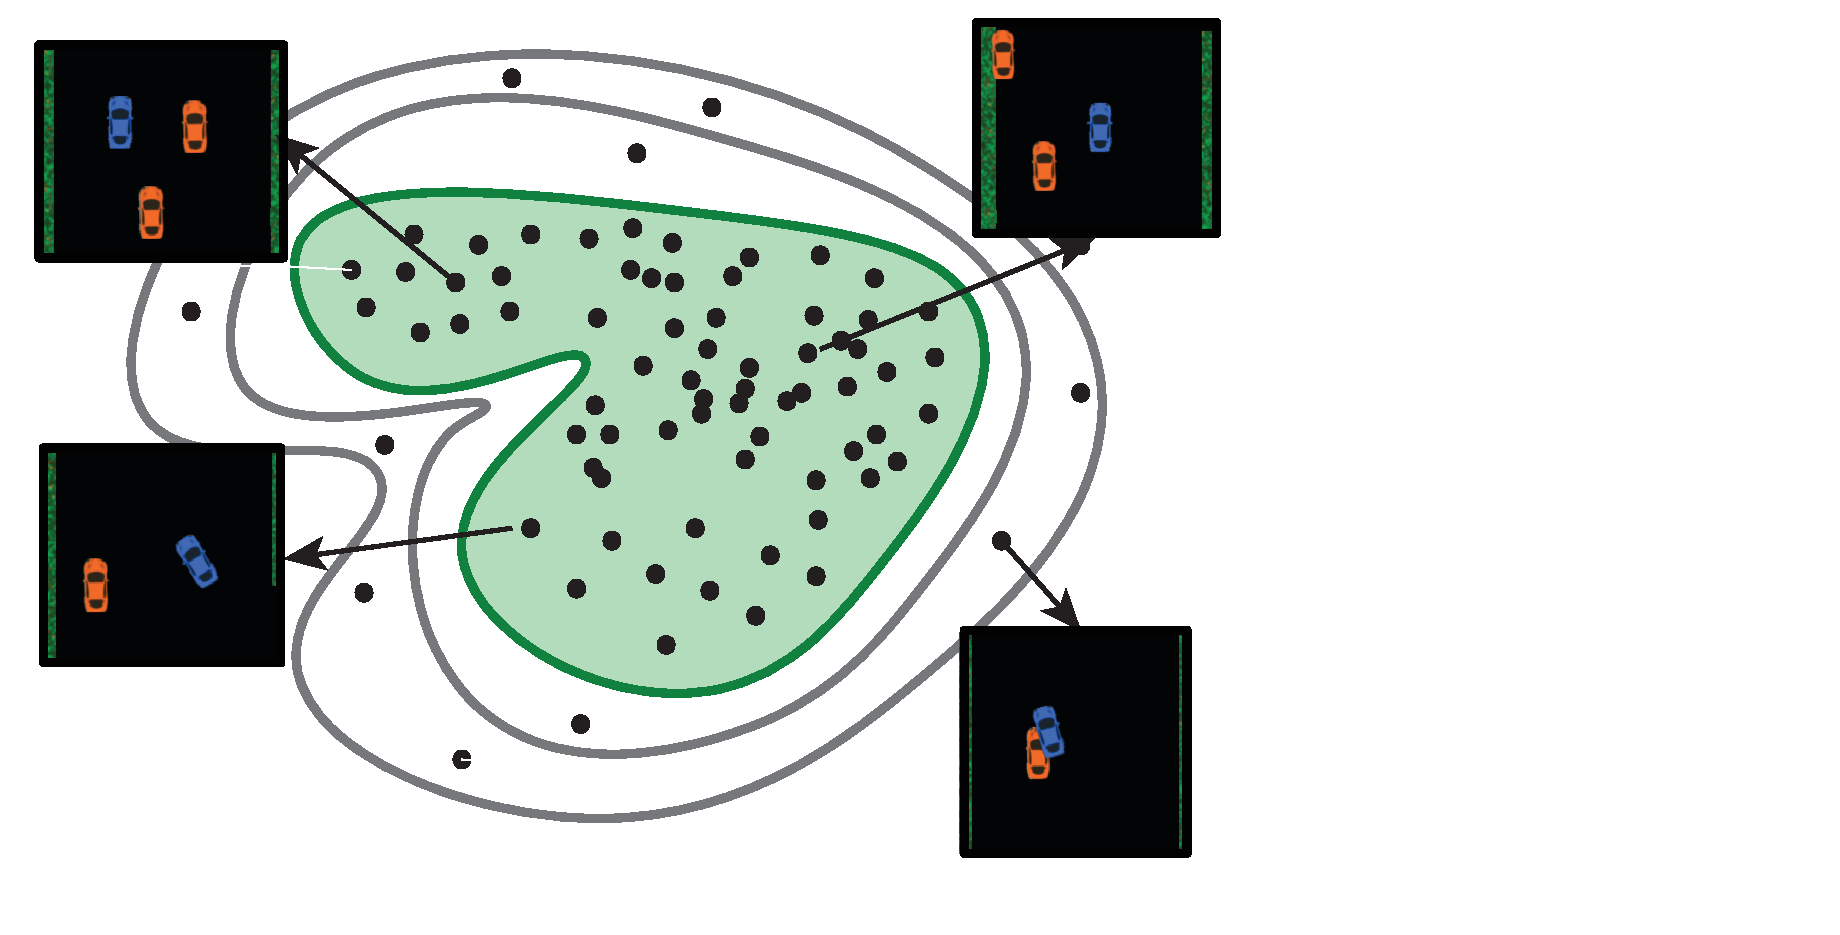
\includegraphics[width=12cm, height=6cm]{figures/teaser.eps}
\caption{ An illustrative example of estimating the risk area in the data collected for a simulated self driving car around a track with other cars. The green area corresponds to points that are likely to occur under the expert demonstrations, where outside are points that would occur with low probability and thus are considered high risk. } 
\vspace*{-10pt}
\label{fig:dis_traveled}
\end{figure}


During learning, implementations of DAgger require the supervisor to manually label the controls the robot should have applied for each states it visits. If the supervisor, is a human this can be tedious and expensive. We are interested in having the supervisor only need to provide labels in areas of high risk, or where the robot is likely to mis-predict the controllers actions to reduce the workload on the controller.  A state can be risky for 2 reasons: 1) its is far from the states trained on, which potentially means our policy will mis-predict the supervisor \cite{tokdar2010importance} 2)  the state in the training set is being mis-predicted, so the state, although visited, doesn't have good control yet 

To estimate where the robot's current policy is likely to mis-predict the supervisor, we  leverage a property in statistical machine learning that a trained model will be able to generalize within the distribution it is trained on \cite{tokdar2010importance}. This property can be seen used in importance sampling when data is collected from one distribution, but tested on another and has to be re-weighted to the test distribution \cite{huang2006correcting}. One approach then is to estimate the distribution the policy is trained on and then ask for the supervisor to take over if the  probability of the current state is low under the estimated distribution. However, the amount of data needed to accurately estimate the density increases exponentially with the dimension of state space \cite{nadaraya1964estimating}. If we are working with partial observations like image data this could be impractical.  Thus, we propose using a modified version of a technique known as the One Class SVM that only tries to estimate the level set of the density trained on \cite{scholkopf2001estimating} and has been shown to successfully work on image data before in the context of outlier detection \cite{liu2014unsupervised}. 

We make the following assumptions access to an environment where a robot can try out policies and sample trajectories and access to a supervisor that is able to provide demonstrations and tell the robot the control it should have applied after each iteration. We also assume that we are able to collect a series of partial observations from the environment and the controls applied. Lastly, we assume the observations encapsulate the Markov assumption in such that the probability of one is only dependent on the last observation and the controls applied. 


Our contributions to date are framing the problem of asking for help in an online setting as estimating the support of a distribution and proposing a modified version of the One Class SVM,that both estimates the level set of a distribution and carves out areas in the support where we know our policy will mis-predict the supervisor, to identify states of high risk.  Initial results on a Mario AI video game, averaged over 20 levels,  suggest SHEATH was able to reach DAgger's peak performance of a distance around 2200 with only 1200 queries to the supervisor, while DAgger required 2800 queries.  \todo{These are preliminary results and I want to test on more mario experiments and the self driving car, also look at robustness to hyperparamters such as $\nu$ before I am confident in them}

\section{Related Work}
The field of learning from demonstration has achieved state of the art performance in a variety of areas within robotics \cite{argall2009survey}. Abbeel et al. used an iLQR controller around helicopter trajectories demonstrated by an expert to successfully learn a series of aerobatics stunts \cite{abbeel2007application}. Billard and Matari used a hierarchy of neural networks on video data and tracking markers to imitate a human arms movements on a 37 degree of freedom humaniod robot \cite{billard2001learning}. Schulman et al. used a non-linear warping, thin plate splines, on collected trajectories of a human controlling a PR2 and tying knots with a rope then transferred the demonstrations to the new unseen initial configurations of the rope~\cite{schulman2013case}. 

 A subset of the learning from demonstration field is working within the assumption of no known dynamics and no access to a cost function. Under these assumptions, one approach to learning from demonstration is to collect a set of trajectories and controls from a supervisor and then treat the problem as a supervised learning problem that regresses on a function from state space to controls~\cite{argall2009survey}. Pomerleau et al. used this approach on raw image data and controls provided by a person driving a car and learned a policy that allowed a car to travel on a highway. However, they observed if the car deviated from the middle of the road it would not know how to recover, this behavior was attributed to the fact the car only drove in middle of the road while collecting demonstrations~\cite{pomerleau1989alvinn}. Ross et al. studied this effect and proved the amount of error accumulated is squared in the time horizon of a policy and proposed a learning algorithm, SMILE, that stochastically mixes the supervisor's control with the robots during training. Thus allowing the robot to explore states the supervisor hasn't seen before~\cite{ross2010efficient}. 

Ross and Bagnell then improved upon this method with DAgger an iterative method that first trains a policy on the data observed using standard supervised learning techniques and tries the policy out in the environment to see what states are likely to occur under the robots policy. The supervisor then tells the robot what controls it should applied after each iteration and the policy is retrained with an aggregate of all data seen before \cite{ross2010reduction}. 

A quad-copter using DAgger learned how to fly through a forest using only HOG features extracted from visual images \cite{ross2013learning}. Guo et al. combined DAgger with Deep Q learning methods to achieve state of the art performance on the common Atari game benchmark in Reinforcement Learning \cite{NIPS2014_5421}. Duvallet use DAgger to teach robots to follow verbal instructions about where to move sematically in a building with a training set of humans following similar verbal instructions \cite{duvallet2013imitation}. Levine et al. extended the iterative learning paradigm through Guided Policy Search, which replaces the expert with iLQG and uses KL divergence constraints to train the policy to match the distributions of the controllers \cite{levine2015end}.  


One limitation of DAgger is that it requires the demonstrator, or supervisor, to "label" every state the policy visits during learning. The act of labeling can be very tedious and expensive when the supervisor is a human. To reduce this Judah et al. proposed applying active learning technique to only query the supervisor for states that are likely to be visited under the current policy and are likely to be mis-predicted under the current policy\cite{judah2011active,judah2012active}. A drawback of this approach though is that it requires estimating the distribution of states, which can be difficult in high dimensions. Furthermore, their use of query by committee reduces their policy's function class to non-kernelized linear classifiers \cite{gilad2005query}, which could potentially hurt the ability of a policy to generalize.
 

In order to tell where a policy is likely to mis-predict,we  leverage a property in statistical machine learning that a trained model will be able to generalize within the distribution it is trained on \cite{tokdar2010importance}. This property is used in importance sampling when data is collected from one distribution, but tested on another and has to be re-weighted to the test distribution \cite{huang2006correcting}. One approach is to  estimate the probability density the policy is trained on. However, the amount of data needed to accurately estimate the density scales exponentially in the number of \cite{nadaraya1964estimating}.

 Several other approaches have been proposed to tell when your estimator is likely to not generalize \cite{2003novelty}.Knox and Ng used a nearest neighbors approach to try and estimate if a point was close to $k$ neighbors, however it was shown to be susceptible to outliers because nearest neighbor only uses local information about the data \cite{knox1998algorithms}. Manevitz and Yousef trained a neural network filter to try and reconstruct the data and if the reconstruction error is high, they mark the point as likely to be outside of the estimators generalization ability. Manevitz and Yousef mention  that finding the right architecture can be task specific and require a lot of hyperparameter tuning  \cite{manevitz2002one}. The One Class SVM proposed by Scholk{\"o}pf et al. estimates a user defined level set of the distribution it is trained on by solving a convex quadratic program   to find the support vectors that encompasses the data. The method has been theoretically shown to approximate the level set of a density estimate in the asymptomatic  limit of sample and also its regularization term has the nice property of being equivalent to the quantile function\cite{vert2006consistency}. It has also been shown to successfully work on outlier detection for raw image data~\cite{liu2014unsupervised}.


\section{Problem Statement}

\subsection{Notation and Background}
\todo{figure out sensor model, meeting with Sergey next week about safe learning with out assuming a human is available I can ask him then}
Define $\mathbf{x} \in \mathcal{X}$ as state space for a robot, for example $\mathbf{x}$ could be an image from a camera feed or a vector of joint angles. Define $\mathbf{u} \in \mathcal{U}$ as the class of controls for an agent, which could be for example torque control applied to a robot or discrete commands such as in a video game. The environment is modeled to have dynamics that are stationary and Markovian, such that the the probability of state $\mathbf{x_{t+1}}$ can be determined from $\mathbf{x}_t$ and $\mathbf{u}_t$, or $p(\bx_{t+1}|\bu_t,\bx_t)$.  We represent a probability distribution over the initial state of the environment $p(\bx_0)$.. Denote a trajectory as series of states visited and the controls applied  as $\tau = (\mathbf{x}_0,\mathbf{u}_1, ...., \mathbf{x}_T,\mathbf{u}_T)$.  A trajectory that is defined with state space only and not controls is $\tau_{\bx} = (\bx_0,....,\bx_T)$.



A policy is a function from state space to controls, $\pi: \bx \rightarrow \bu$. A policy could be $\pi_\theta: \bx \rightarrow \mathbf{u}$, which is a  function that is specified by a vector of parameters  $\theta$.The vector of parameters $\theta$ can be for example weights in a neural network or the  vectors in a Support Vector Machine. A policy, $\pi_{\theta}$ in an environment with $p(\bx_0)$ and $p(\bx_{t+1}|\bx_t,\bu_t)$ induces a distribution on the possible trajectories:$ p(\tau_\bx | \theta)= p(\bx_0)\prod_{i=0}^{T-1}p(\bx_{t+1}|\pi_{\theta}(\bx_t),\bx_t)$. Also $\pi_{\theta}$ in an environment with $p(\bx_0)$ and $p(\bx_{t+1}|\bx_t,\bu_t)$  induces a distribution on states visited $p(\mathbf{x}|\theta)$. 

 The following is a way to convert from $p(\bx_t|\theta)$ to $p(\bx|\theta)$. Let $p(\bx_t|\theta)$ be the distribution of states visited at time $t$ if the robot follows the policy $\pi_{\theta}$ for $t-1$ time steps. Calculating this from $p(\tau_{\bx}|\theta)$ is mean marginalizing over the previous timesteps $p(\bx_t|\theta) = \int_{\bx_{t-1}}...\int_{\bx_1} p((\bx_t,...,\bx_1)|\theta) d\bx_{t-1}...d\bx_1$. The average distribution on states is now defined as $p(\bx|\theta) = \frac{1}{T} \sum^T_{t=1} p(\bx_t|\theta)$.



We do not know the distributions: $p(\bx_{t+1}|\bx_t,\bu_t)$, $p(\bx_0)$,$p(\tau_{\bx}|
\bx)$ or $p(\bx|\theta)$. But we assume we have a stochastic real robot or a simulator such that given any state $\bx_t$ and control $\bu_t$, it will move into a state $\bx_{t+1}$ such that $\bx_{t+1} \sim p(\bx_{t+1}|\pi_{\theta}(\bx_t),\bx_t)$. Note that $p(\tau_{\bx}|\theta)$ is high dimensional because $\bx$ is high dimensional. 

Given $\pi_{\theta}$ we want to identify a set of highly probable trajectories and the associated highly probable states. We assume we are given some initial state $\bx_0$. We  "roll-out" the policy using the robot with the policy to sample the resulting trajectory and set of states reached, which provides a sequence of highly probably states under $p(\tau_{\bx}|\theta)$.Rather than estimating $p(\bx|\theta)$ or $p(\tau_{\bx}|\theta)$, we draw samples from them. 


The objective in policy learning can be framed as minimizing some cost function $C(\tau) = \sum^T_{t=1} c(\bx_t,\bu_t)$. The cost function is user defined and task specific. For each state $\bx_{t}$ and control $\bu_t$ the robot receives a penalty related to how far it is from the goal state. For example, in task of inserting a peg into a hole the cost function can be distance to desired final state \cite{levine2015end}.  We also do not know the cost function. But we do have access to a "supervisor", an algorithm or human that uses some policy $\tilde{\pi}$ to minimize $C(\tau)$, and we are given an initial set of $N$ training/demonstration trajectories resulting from this policy: $\mathcal{D} = \lbrace \tilde{\tau}^1,...,\tilde{\tau}^N \rbrace$. 

Next, we define a "surrogate" loss function $l$, which gives the distance between any pair of control values: in the continuous case $l(\bu_0,\bu_1) = ||\bu_0-\bu_1||^2$ or in a discrete case

 \vspace{-2ex}
\begin{align}
 l(\bu_0,\bu_1) = \left\{
     \begin{array}{lr}
       1 & : \bu_0 = \bu_1\\
       0 & : \bu_0 \neq \bu_1
     \end{array}
   \right.
\end{align}

Given a candidate policy $\theta$, we can use the surrogate loss function to compute how "close" it is to the supervisor's policy $\tilde{\pi}$. 

We want to compute a policy $\pi_{\theta}$ that minimizes the expected surrogate loss where the expectation is taken over the distribution of states. 

 \vspace{-2ex}
\begin{align}\label{eq:LFD_obj}
\underset{\theta}{\min} \: E_{p(\bx|\theta)} [l(\pi_\theta(\bx),\tilde{\pi}(\bx))]
\end{align}
 
 
 
 
The optimization problem in Eq. \ref{eq:LFD_obj} compares the action taken of the policy $\pi_\theta$ and  the supervisor, $\tilde{\pi}$  weighted by the probability of  the state occurring $p(\bx|\theta)$. 

Eq. \ref{eq:LFD_obj} is hard to solve because  the objective is not convex and we only have access to $\tilde{\pi}(x)$, where $x$ is a state in one of the demonstrations or $\bx \in \mathcal{D}$. To address these issues Stephane and Ross proposed an iterative method known as DAgger\cite{ross2010reduction}.






 \subsection{DAgger: Dataset Aggregation}
 DAgger is an iterative algorithm that repeats two steps for $K$ iterations. 
 In Eq. \ref{eq:LFD_obj}, the objective involves both the parameterized policy $\pi_{\theta}$ and the average distribution of states with respect to the policy, $p(\bx|\theta)$. DAgger iteratively minimizes $\pi_{\theta}$ on the collected dataset of examples $\mathcal{D}$ and then adds new states of high probability under $\pi_\theta$ by sampling via policy roll outs from $p(\bx|\theta)$. 

\subsubsection{Step 1}
At iteration $k=0$ given a dataset $\mathcal{D}_0$, the training set with $N_0$ demonstrated trajectories mapping $\bx$ to $\bu$. DAgger solves the following supervised learning problem with respect to the surrogate loss function. 

 \vspace{-2ex}
\begin{align}\label{eq:super_objj}
\theta_{k} = \underset{\theta}{\argmin} \: \sum_{i=1}^{N}\sum_{t=1}^T l(\pi_{\theta}(\bx_t^{i}),\bu_{t}^i)
\end{align}
 
 
This is a supervised learning problem and can be solved using standard machine learning techniques, for example a support vector machine or a neural network. The surrogate losses mentioned early like Squared Euclidean distance or an Indicator function are appropriate optimization objectives. 
 
 To handle the fact that the supervisor's policy contains noise $\epsilon$, we employ a regularization technique in the optimization. Regularization is a technique to control the smoothness of the function that is fit to the sampled data. It is a common technique to make the estimator robust to zero mean noise on data. In practice it is a penalty term on either  the L2 norm on the weights for regression based techniques or the slack coefficient for support vector machines \cite{scholkopf2002learning}.
 
 \subsubsection{Step 2}
DAgger rolls out the policy $\pi_{\theta_{k=1}}$ to sample states that are likely to occur under $\theta_{k=1}$. For every state visited, DAgger requests the supervisor to provide the appropriate control/label. Formally, for a given sampled trajectory  $\tau = (\bx_1,\bu_1,...,\bx_T,\bu_T )$. The supervisor provides labels $\tilde{\bu}_t$, where $\bu_t \sim \pi(\bx_t) + \epsilon$ to the trajectory $\tau = (\bx_1,\tilde{\bu}_1,...,\bx_T, \tilde{\bu}_T )$.  This can be very tedious for a human. The states and labeled controls are then aggregated into the next data set of demonstrations $\mathcal{D}_1$. 


Steps 1 and 2 are repeated for $K$ iterations or until the cumulative surrogate loss  goes to zero. Since DAgger requires rolling out the policy at each iteration, one way to terminate the algorithm is when the performance of the rolled out policy matches the intended behavior, or more formally when the surrogate loss is below some predefined threshold $\gamma$.  


Dagger works well in both simulation and real world experiments. It also has theoretical guarantees that it will converge in the limit to the supervisor's policy. However, using policy rollouts means the robot can enter dangerous states, which could damage a robot in a non simulation system. For example, when DAgger was used on a quad-copter the robot repeatedly crashed into trees before successfully learning to avoid them \cite{ross2013learning}. A state can be risky for 2 reasons: 1) its is far from the states trained on, which potentially means our policy will mis-predict the supervisor and incur high surrogate loss \cite{tokdar2010importance} 2) the surrogate loss associated with the state is high, so the state, although visited, doesn't have good control yet. Furthermore, iterations are tedious because if a human is the supervisor requires manual "labeling" of every state visited with the appropriate control. 

To address these limitations, we propose to 1) avoid highly risky states entirely via terminating the policy roll-out and 2) recognize slightly risky states and request human input for these and to reduce the burden on the human trainer. One way to do this is to define risk in terms of distance to the nearest neighbor, but this vulnerable to outliers in the known set of states. Another option is to fit a distribution to the known set of states, which requires an exponential number of samples in the dimension of the state space \cite{nadaraya1964estimating}. We propose using a modified version of the technique known as the One Class SVM that  estimates a boundary of the density \cite{scholkopf2001estimating}.


\subsection{Estimation of a Distribution's Level Set}\label{sec:level}
\todo{Work with Florian on the first paragraph to make it less abstract and specific to the robotics}
Support estimation can be defined as minimizing a function that contains the volume of a given probability distribution. Formally we define it as follows let $\mathbf{x}_1,...,\mathbf{x}_n $ be i.i.d. random variables in a set $\mathcal{X}$ with distribution $P$. Let $\mathcal{G}$ be a class of measurable subsets of $\mathcal{X}$ and let $\lambda$ be a real function defined on $\mathcal{G}$. The quantile function with respect to $(P,\lambda,\mathcal{G})$ is 

\vspace{-2ex}
\begin{align}\label{eq:quantile}
U(\gamma) = \mbox{inf} \lbrace \lambda(G):P(G) \geq \gamma, G \in \mathcal{G} \rbrace \: 0<\gamma \leq 1
\end{align} 


We denote by $G(\gamma)$ the $G \in \mathcal{G}$ that attains the infinimum. The most common choice of $\lambda$ is Lebesgue measure, in which case $G(\gamma)$ is the minimum volume $G \in \mathcal{G}$ that contains at least a fraction $\gamma$ of the the probability mass. Thus, $G(1)$ is the support of the density $p$ corresponding to $P$, assuming it exists. 

To handle high dimensional densities $P$, work by Scholk{\"o}pf et al.  looked at representing the class $\mathcal{G}$ via a kernel $k$ as the set of half-spaces in the support vector (SV) feature space \cite{scholkopf2001estimating}. They then minimize a SV  regularizer which, using a kernel, controls the smoothness of the estimated function describing $G$. In terms of the quantile function described in Eq. \ref{eq:quantile}, the approach can be thought of as employing $\lambda(G) = ||w||^2$, where $G_w = \lbrace x: f_w(x) \geq \rho \rbrace$. Here $(w,\rho)$ are a weight vector and offset parameterizing a hyperplane in the feature space associated with a kernel. 


\begin{figure*}[ht]
\centering
\subfigure[Race Car Simulator]{%
\vspace{-0.5ex}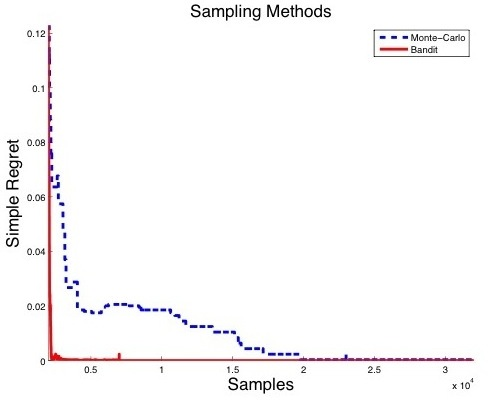
\includegraphics[width=5cm , height = 4cm]{figures/Slide1.jpg}
\label{fig:subfigure1}}
\quad
\subfigure[Expert Demonstrations]{%
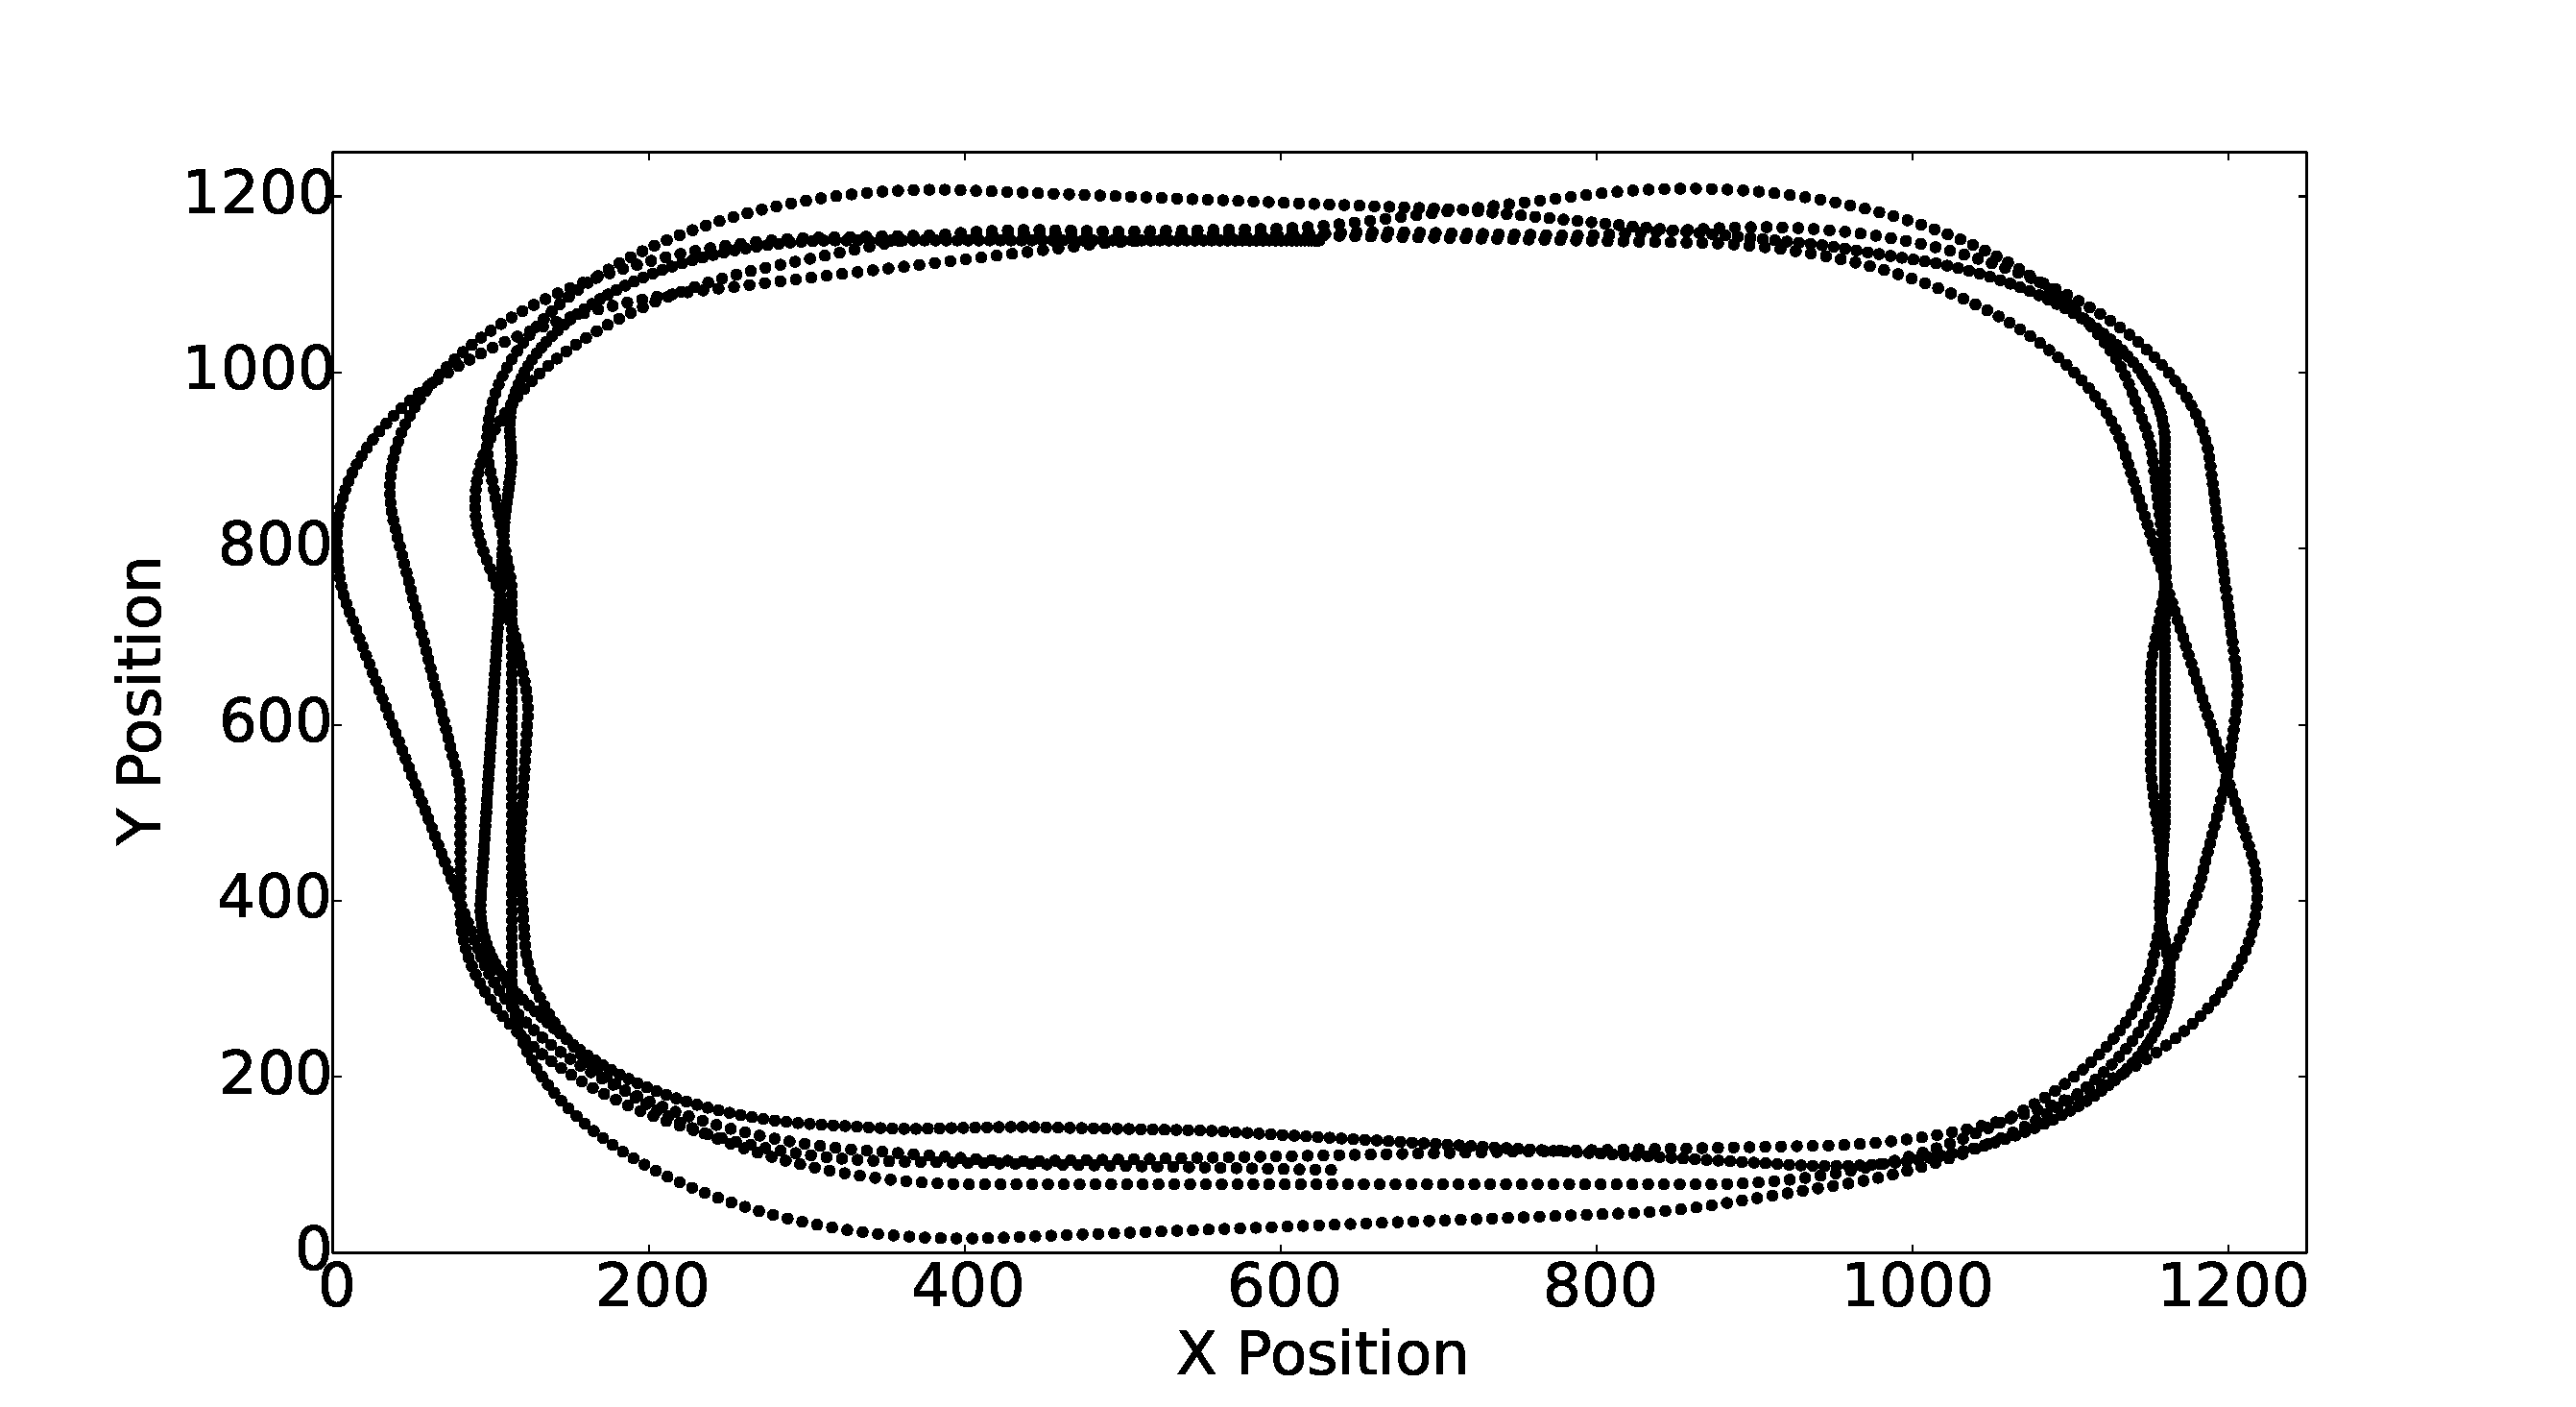
\includegraphics[width=5.5cm, height = 4.5cm]{figures/exp_dist.eps}
\label{fig:subfigure2}}
\subfigure[Estimated Support of Expert Demonstrations]{%
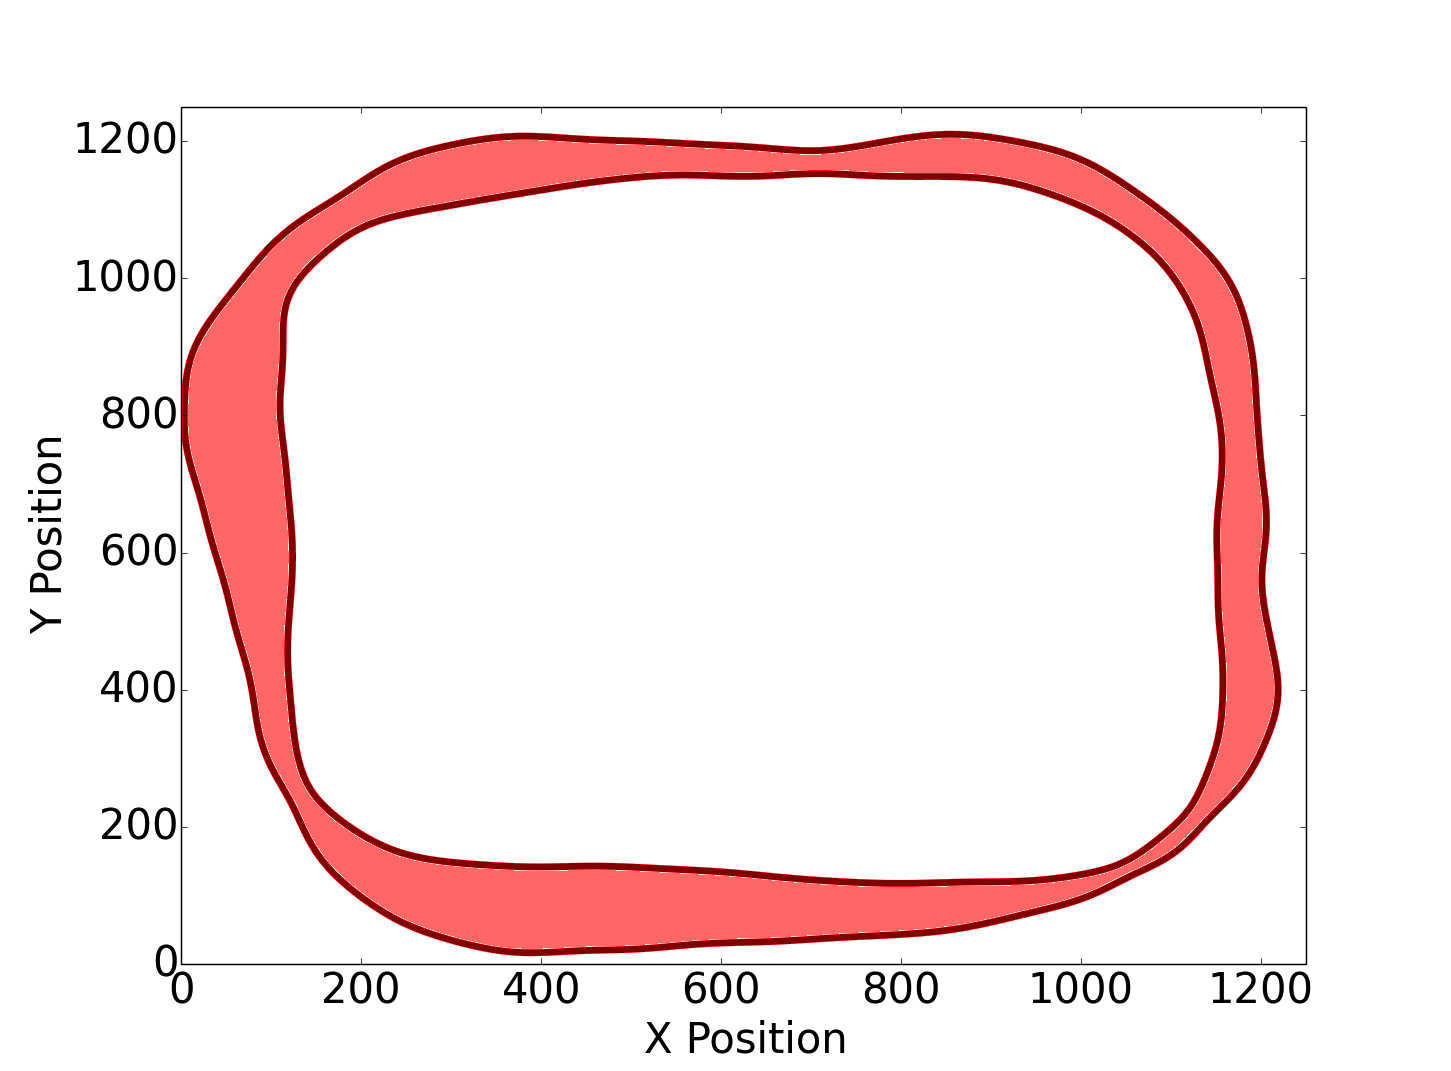
\includegraphics[width=5.5cm, height = 4.5cm]{figures/ocm_example.png}
\label{fig:subfigure3}}

\caption{\todo{Want to change this to highlight $\nu$ effect on level set estimation} A race car is driven around a track in Fig. \ref{fig:subfigure1} by an expert demonstrator. The state space of the car is represented as the x and y positions on the track or $\mathbf{s} = [x,y]$. In Fig. \ref{fig:subfigure2}, the demonstrations are plotted in state space. In Fig. \ref{fig:subfigure3}, the support is estimated using the decision function in \ref{eq:decision_func}. As illustrated the support accurately describes the boundary of the expert trajectory. }
\label{fig:support_example}
\end{figure*}


Let $\Phi$ be a feature map $\mathcal{X} \rightarrow \mathcal{F}$, i.e. a map into an inner product space $\mathcal{F}$ such that the inner product in the image of $\Phi$ can be computed by evaluating some  kernel

\vspace{-2ex}
\begin{align}
k(\bx_0,\bx_1) = \langle\Phi(\bx_0),\Phi(\bx_1)\rangle
\end{align}

such as the Gaussian kernel 

\vspace{-2ex}
\begin{align}
k(\bx_0,\bx_1) = e^{-||\bx_0 - \bx_1||^2/c}
\end{align}

The main idea is to solve an optimization problem that separates the origin, we solve the following quadratic problem:

\vspace{-2ex}
\begin{align}\label{eq:primal_sup}
\underset{w\in F, \mathbf{\xi} \in \mR, \rho \in \mR}{\mbox{min}}\: \frac{1}{2}||w||^2+\frac{1}{vn} \sum^n_i \xi_i - \rho\\
\mbox{s.t} \: \langle w,\Phi(x_i) \rangle \geq \rho - \xi_i, \: \xi_i \geq 0 \notag
\end{align}

The parameter $\nu$ controls the penalty on slack terms and asymptotically approaches is equivalent to $\gamma$ \cite{vert2006consistency}.  The decision function then becomes 

\vspace{-2ex}
\begin{align}\label{eq:decision_func}
g(x) = \mbox{sgn}(\langle w,\Phi(x) \rangle-\rho)
\end{align}

Where $g(x) = 1$ indicates in the support region and $(g) = -1$ denotes being outside the support region. The dual form of the optimization takes the form of a Quadratic Program with respect to the Gram Matrix \cite{scholkopf2001estimating}. 

Estimating the level set of a distribution can be a measure of the generalization ability of $\pi_{\theta}$ to points not within $\mathcal{D}$. However, it does not account for the fact that for a given $\theta$ or  solution to Eq. \ref{eq:super_objj}. $\pi_\theta$ may not correctly match the supervisor's controls for all points train on. To account for this, we propose a modification to the One Class SVM denote: 

\begin{align}
y_i = \left\{
     \begin{array}{lr}
       1 & : \pi_{\theta}(\bx_i) =\bu_i\\
       -1 & : \pi_{\theta}(\bx_i) \neq \bu_i
     \end{array}
   \right.
\end{align}

or $y_i$ is $1$ if the control applied matches the supervisor and $-1$ if it differs. In the regression case the decision between $1$ and $-1$ can be set by a some threshold on a L2-norm or $||\pi_{\theta}(\bx_i)-\bu_i||$. We use $y_i$ to modify the optimization as follows: 

\vspace{-2ex}
\begin{align}\label{eq:primal_sup}
\underset{w\in F, \mathbf{\xi} \in \mR^l, \rho \in \mR}{\mbox{min}}\: \frac{1}{2}||w||^2+\frac{1}{vn} \sum^n_i \xi_i - \rho\\
\mbox{s.t} \: y_i \langle w,\Phi(x_i)\rangle \geq \rho - \xi_i, \: \xi_i \geq 0 \label{eq:ineq}
\end{align}

Points that are mis-predicted are then enforced to lie on the opposite of the hyper-plane in the feature space $\phi(\bx)$, which carves out holes in the support region around them. The dual formulation, which is what is solved in practice, can be derived as 

\vspace{-2ex}
\begin{align}\label{eq:dual_sup}
\underset{\alpha\in \mathcal{R}}{\mbox{min}} \sum_i^n \sum_j^n \alpha_i\alpha_j y_i y_jk(\bx_i,\bx_j)\\
\mbox{s.t} \: 0 \leq \alpha \leq \frac{1}{\nu n} \:, \sum_i^n \alpha_i = 1 
\end{align}

Our decision boundary function $g(\bx)$ is then derived in terms of the support vectors as $g(\bx) = \sum_i^n \alpha_i y_i k(\bx_i,\bx) - \rho$. To compute the $\rho$ term,we leverage the fact that for an optimal solution the inequalities in Eq. \ref{eq:ineq} are equal for any $\alpha_j$ such that $0 < \alpha_j < \frac{1}{\nu n}$. Therefore we can compute $\rho$ as  $\rho = \sum_i^n y_i \alpha_i k(\bx_i,\bx_j)$ \cite{scholkopf2001estimating}. 




\subsection{SHEATH:Support-based HElp AquisiTion from Humans}

Our proposed method trains a policy, $\pi_{\theta_k}$, but also estimates where the policy is likely to accurately predict the supervisor's control,which we define as the region of low risk.  In the statistics community, a known property is that estimators are function will likely mis-classify if they are evaluated at points not in the distribution sampled from.Techniques such as importance sampling use this results to train estimators on data drawn from a different distribution \cite{tokdar2010importance}.  Thus, we try to estimate the level set of the training distribution, which is explained in \ref{sec:level} and only have the supervisor provide labels when the robot leaves this boundary. Furthermore to avoid entering pathological states that are far from the supervisor's demonstrations, we terminate the roll-out when it is a certain distance or risk factor from the decision boundary, which is given by $r(\bx) = \sum_i^n \alpha_i \bx_i k(\bx_i,\bx)-\rho$. The risk threshold, $r_0$, is user defined based on the task. 

\subsubsection{Step 1}
Similar to DAgger at iteration $k$ the algorithm estimates a policy, $\pi_{\theta_k}$ on the dataset $\mathcal{D}_k$ by solving Eq. \ref{eq:super_objj}. We then estimate the level set of the distribution being trained on by solving the optimization for the One Class SVM or $\ref{eq:primal_sup}$ on the dataset $\mathcal{D}_k$. We now have a decision boundary $g_k(\bx)$, which is $1$ if the region is in the low risk area and $-1$ otherwise . The parameter $\nu$ is an estimate of how much probability mass is contained in the level set and can be use to control the size of the low risk region. 
 
 
 \subsubsection{Step 2}
 In DAgger the policy that was rolled out is $\pi_{\theta_k}$, however this could potential encounter pathological states that are far from the initial set of demonstrations $\mathcal{D}_0$. To prevent this we terminate the rolled out policy if the risk, or distance from the support, is above some threshold $r(\bx_t) > r_0$.  Furthermore, instead of labeling every state now the supervisor is only require to label states outside of the level set or $\bx$, where $g(\bx) = -1$.  These states are then added to the dataset $\mathcal{D}_{k+1}$ and the algorithm goes back to Step 1. 

An implicit trade off exists between what how much of the distribution is contained in the selected level set and the amount of exploration the robot is allowed. If the level set is large the robot will be allowed to explore in this region and potentially make more mistakes with respect to the expert, but learn faster. If the level set contains a smaller fraction of data, then the expert will be in control more and the robot will learn at a slower rate. 


\section{Theoretical Analysis}

\subsection{Convergence Rate}
\todo{These are ideas still in progress}
The convergence rate of DAgger is dependent on the probability of the expert taking over at each iteration $\beta_i$ \cite{ross2010reduction}. For SHEATH, this corresponds to the probability of leaving the support or $p(g(\mathbf{x}) = -1|\pi_{\theta_i})$ . The intuition is that the larger the level set parameter $\nu$ is the lower the probability of leaving is and thus faster convergence rate, but potentially less safe exploration. Not sure if a formal proof is going to be possible though with assuming known dynamics, still looking into it. However, we can experimentally demonstrate this. 




\section{Experiments}
\subsection{Driving Example}
A common benchmark in RL is a car driving around a track avoiding other cars \cite{argall2009survey}. In our driving simulator, the car must stay on a rectangular track and dodge the orange cars that are on the track as well. If the car falls off the track, it is placed back on to the center. The car's control space $u = \lbrace -15^\circ, 0, 15^\circ \rbrace$ or 3 discrete commands that change the angle of the car. The internal state space of the car is xy-coordinates and the angle it is facing. Our supervisor is a solver that uses state space search through the driving simulator to plan the next control.

We have the supervisor drive around the track 2 times and then collect the raw images observed. We use a Gaussian Pyramids to down sample the images to $125 \times 125$ RGB pixels and then extract Histogram of Oriented Gradients (HOG) features using OpenCV. For both DAgger and SHEATH, we use a Linear Support Vector Machine (SVM) as the policy representation, with the regularization term on the slack variable $\gamma=0.01$, which was set via cross validation on the initial training examples from our expert. For the optimization of Eq. \ref{eq:dual_sup} in SHEATH we used a radial basis function as well for the kernel with a bandwidth of $\lambda=0.01$ and $\nu = 0.95$ to account for $95\%$ of the training distribution. 

We compare performance in terms of minimization of the underlying cost function $c(\bx,\bu)$, which is the sum of the number of times the car left the track and the number of times the car collided with the other cars on the track, versus the number of queries made to the supervisor. Initial results averaged over 1 level shown in Fig.  suggest an $75\%$ reduction in the number of queries needed for SHEATH compared to DAgger. 




\begin{figure}[t!]
\centering
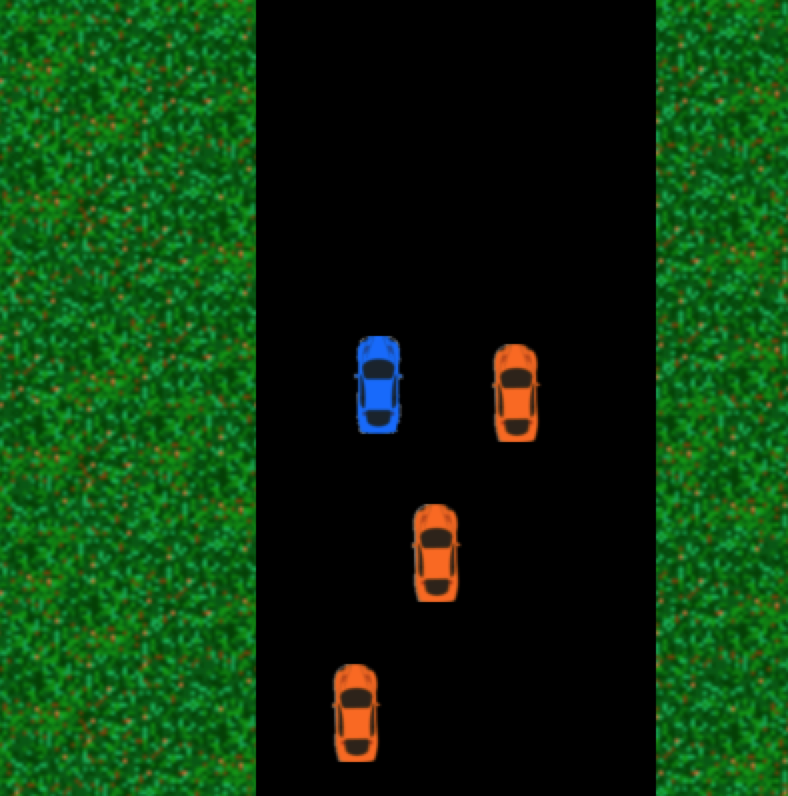
\includegraphics[width=6cm, height=6cm]{figures/race_car_track_example.png}
\caption{ An example image from the racing simulator. The car is meant to drive around a rectangular track and dodge other cars. The supervisor drives around the track for 3 iterations and HOG features are extracted from the images.  }

\vspace*{-10pt}
\label{fig:race_car}
\end{figure}


\begin{figure}[t!]
\centering
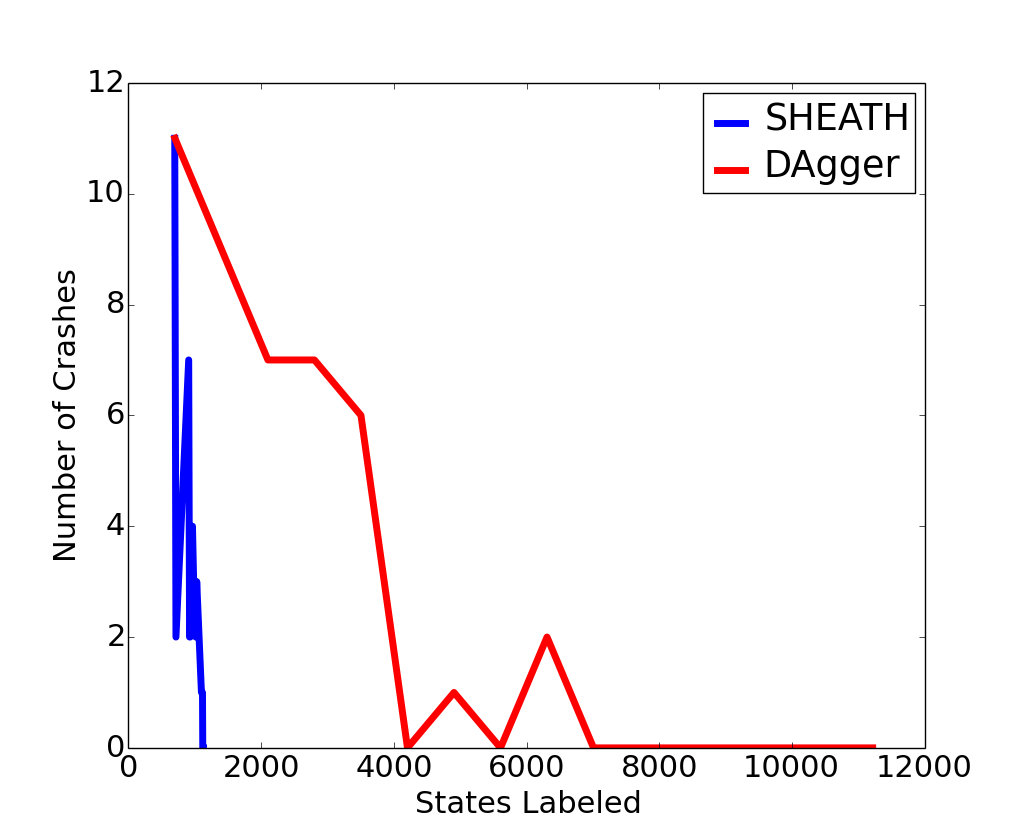
\includegraphics[width=8cm, height=6cm]{figures/dagger_sheath_no_cars.png}
\caption{ We compare performance in terms of optimization of the underlying cost function $c(\bx,\bu)$, which is the sum of the number of times the car left the track and the number of times the car collided with the other cars on the track. Initial results averaged over 1 level shown suggest an $75\%$ reduction in the number of queries needed for SHEATH compared to DAgger. \todo{Run this over many trials}  }

\vspace*{-10pt}
\label{fig:car_cost}
\end{figure}


\subsection{Super Mario Bros}
Super Mario Bros. is a platform video game where the character, Mario, must move across each stage by avoiding being hit by enemies and falling into gaps, and before running out of time. We used the simulator from a recent Mario Bros. AI competition which can randomly generate stages of varying difficulty (more difficult gaps and types of enemies) \cite{marioAI}. Our goal is to train the computer to play the game based on current game features as input. Our expert is a near optimal $A^*$ search algorithm that plans ahead using the game simulator. An action consists of 4 binary variables indicating which subset of buttons we should press in $\lbrace \mbox{left},\mbox{right},\mbox{jump},\mbox{speed} \rbrace$. For both DAgger and SHEATH, we use a Linear Support Vector Machine (SVM) as the policy representation, with the regularization term on the slack variable $C\gamma=0.01$, which was set via cross validation on the initial training examples from our expert.. We initialized both Dagger and SHEATH with two expert demonstrations for each level. For the optimization of Eq. \ref{eq:dual_sup} in SHEATH we used a radial basis function as well for the kernel with a bandwidth of $c=0.01$ and $\nu = 0.95$ to account for $95\%$ of the training distribution. 

\begin{figure}[t!]
\centering
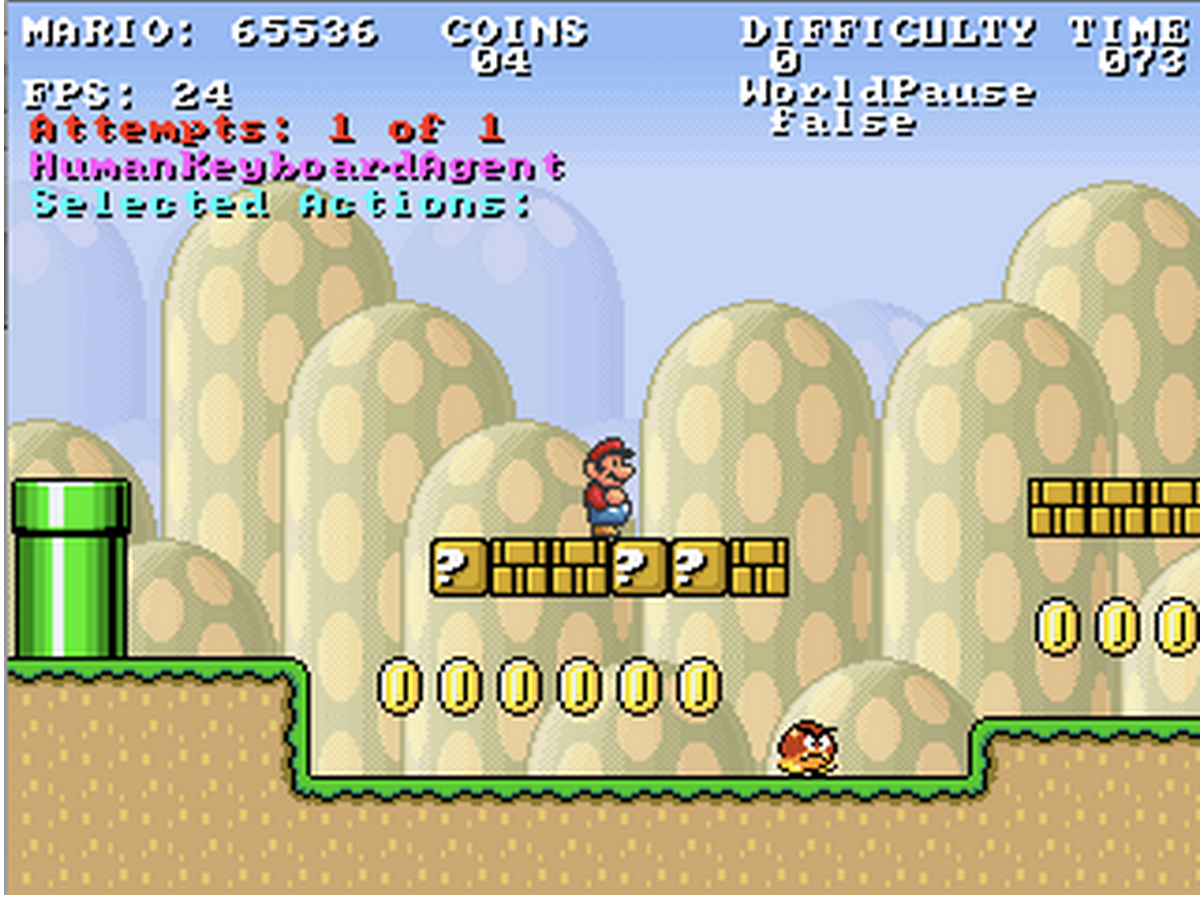
\includegraphics[width = 6cm ]{figures/mario.png}
\caption{ An example image from the Mario AI simulator. Mario faces many challenges to reach an end of a level, such as gaps, jumps and enemies.  }

\vspace*{-10pt}
\label{fig:dis_traveled}
\end{figure}



\begin{figure}[ht]
\centering

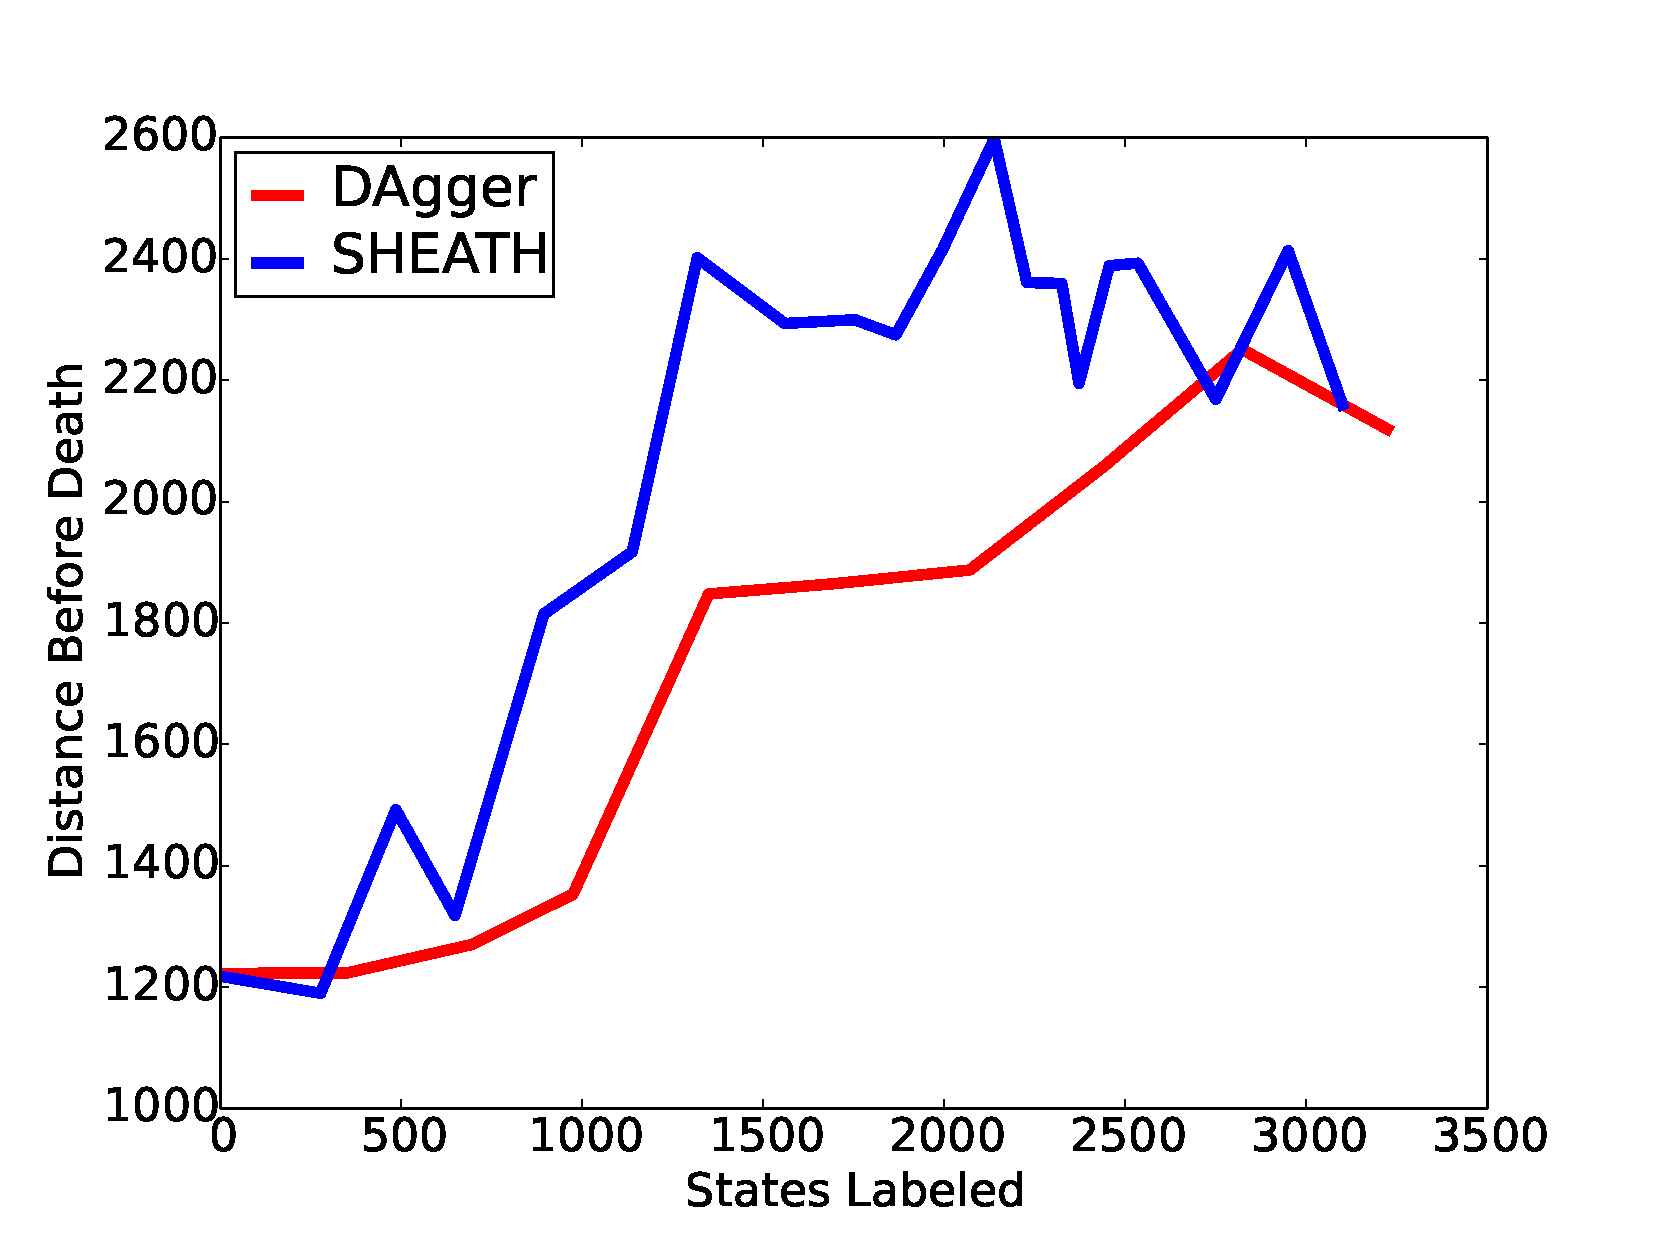
\includegraphics[width=8cm, height = 4.5cm]{figures/dagger_sheath_mario.eps}


\caption{We compare performance in terms of average distance traveled by Mario per stage before dying, running out of time or completing the stage, on randomly generated stages of difficulty 1 with a time limit of 35s to complete the stage.  Stages of difficulty 1 are fairly easy for an average human player but contain most types of enemies and gaps, except with fewer enemies and gaps than stages of harder difficulties. We compare performance of our method and DAgger. In Fig. \ref{fig:mario_results}, we report the performance of distance traveled vs. the number of labels provided by the supervisor. Initial results, averaged over 20 levels, suggest SHEATH was able to reach DAgger's peak performance of a distance around 2200 with only 1200 labels, while DAgger required 2800.   \todo{I think these results are promising but want to make clear they are very preliminary and want to run more experiments on Mario and the self driving car to ensure that we can actually do this reliable. Also, the jaggedness is concerning and needs to be looked in to, my intuition is telling me that Mario is just a very chaotic environment though. I am going to average over more levels to see if it improves}}
\label{fig:mario_results}
\end{figure}

We compare performance in terms of average distance traveled by Mario per stage before dying, running out of time or completing the stage, on randomly generated stages of difficulty 1 with a time limit of 35s to complete the stage.  Stages of difficulty 1 are fairly easy for an average human player but contain most types of enemies and gaps, except with fewer enemies and gaps than stages of harder difficulties. We compare performance of our method and DAgger. In Fig. \ref{fig:mario_results}, we report the performance of distance traveled vs. the amount of time a level was tried.  Initial results, averaged over 20 levels,  suggest SHEATH was able to reach DAgger's peak performance of a distance around 2200 with only 1200 labels, while DAgger required 2800.  



\subsection{Other Experiment}
\todo{Florian and I are discussing different ideas for this one, maybe a controller for an arm or something along the lines of learning to grasp in clutter}


\section{Discussion and Future Work}


\bibliographystyle{IEEEtranS}
\bibliography{references}



\end{document}
